\documentclass[11pt,a4paper]{article}

\usepackage[utf8]{inputenc}
\usepackage[T1]{fontenc}
\usepackage[french]{babel}
\usepackage{lmodern}
\usepackage[top=2.5cm,bottom=2.5cm,left=2.7cm,right=2.7cm]{geometry}
\usepackage{amsmath,amssymb,amsthm,mathtools}
\usepackage{graphicx}
\usepackage{booktabs,array}
\usepackage[dvipsnames]{xcolor}
\usepackage{hyperref}
\hypersetup{colorlinks=true,linkcolor=NavyBlue,citecolor=NavyBlue,urlcolor=NavyBlue,
  pdftitle={CTP Core v2.0 : réputation à témoins responsables},pdfauthor={Ange AWALA}}
\usepackage[font=small,labelfont=bf]{caption}

\theoremstyle{plain}
\newtheorem{proposition}{Proposition}
\newtheorem{corollaire}{Corollaire}
\theoremstyle{definition}
\newtheorem{definition}{Définition}
\newtheorem{hypothese}{Hypothèse}
\newtheorem{regle}{Règle}
\theoremstyle{remark}
\newtheorem{remarque}{Remarque}

\newcommand{\CTP}{\textsc{ctp}}
\newcommand{\clip}{\operatorname{clip}}
\newcommand{\1}{\mathbf{1}}
\newcommand{\E}{\mathbb{E}}
\newcommand{\Prob}{\mathbb{P}}

\title{\textbf{Un mécanisme de réputation à témoins responsables~:\\
modèle, calibration et évaluation du CommunityTrust Protocol\\(\CTP{} Core v2.0)}}
\author{Ange AWALA\\
\small OpenScience Community --- ORCID 0009-0006-0220-3006\\
\small \texttt{openscience.community@proton.me}}
\date{\small Prépublication --- version 2.0 --- non relue par les pairs}

\begin{document}
\maketitle

\begin{abstract}
\noindent
Les groupes d'épargne rotative (tontines) fonctionnent sans garantie formelle
parce que leurs membres observent mutuellement leur fiabilité passée. Nous
étudions un mécanisme de réputation numérique inspiré de cette logique~: le
score d'un membre évolue selon ses contributions, ses défauts d'engagement et
son inactivité, et une contribution n'est comptabilisée qu'après approbation
par un panel de \emph{témoins} tirés au sort qui engagent leur propre score.
Nous corrigeons le modèle publié en v0.1 et v1.1, qui contenait des erreurs
démontrables, et établissons des conditions fermées pour la tolérance au
défaut, la capture d'un panel par une coalition, la rentabilité de la
collusion, l'incitation à contribuer au score maximal, le dilemme du
vérificateur et le coût d'entrée d'une identité. Ces conditions fournissent une
méthode de calibration. Évalué par simulation (jusqu'à 200 graines par
configuration) contre deux références --- audit seul et témoins sans
responsabilité ---, avec des agents qui apprennent à frauder et à valider sans
vérifier, et sous une analyse de sensibilité, le mécanisme recalibré
rend la collusion perdante pour des coalitions allant jusqu'à la moitié des
membres, alors que l'audit seul laisse passer $85\,\%$ des fraudes au même
taux d'audit. Avec des agents adaptatifs, il maintient fraude et validation
sans vérification au niveau de l'exploration, là où les règles de v1.1 ou
l'absence de responsabilité des témoins conduisent à un effondrement (plus de
$90\,\%$ de fraude). L'analyse de sensibilité a révélé deux défaillances ---
erreurs d'audit et petits groupes ---, corrigées par un contre-audit et un panel
adaptatif, ainsi qu'une condition d'applicabilité~: la précision des témoins.
Nous décrivons enfin une instanciation pour les tontines (paiements
vérifiables, ordre de rotation par score, parrainage) et un protocole de
collecte de données pour sa calibration empirique, qui reste à réaliser.

\medskip\noindent
\textbf{Mots-clés~:} systèmes de réputation, tontines, ROSCA, collusion,
attaque Sybil, dilemme du vérificateur, conception de mécanismes,
simulation multi-agents.
\end{abstract}

% ════════════════════════════════════════════════════════════════
\section{Introduction}
% ════════════════════════════════════════════════════════════════

Les associations rotatives d'épargne et de crédit (ROSCA), appelées tontines en
Afrique de l'Ouest, rassemblent des membres qui versent périodiquement une
cotisation dont la somme est attribuée à tour de rôle à l'un d'entre
eux~\cite{ardener1964,besley1993,handa1999}. Leur faiblesse structurelle est
connue~: un membre qui a déjà reçu le pot est incité à cesser de cotiser, et
l'exécution des engagements repose sur la pression sociale et la menace
d'exclusion~\cite{anderson2009}. La réputation --- la mémoire collective du
comportement passé --- est donc le mécanisme central.

Les systèmes de réputation numériques cherchent à reproduire cette mémoire à
grande échelle~\cite{resnick2000,dellarocas2003,josang2007}. Ils se heurtent à
des difficultés bien documentées~: manipulation par des coalitions, identités
multiples (attaque Sybil~\cite{douceur2002}), blanchiment de réputation par
changement d'identité~\cite{friedman2001}, et paresse des
vérificateurs lorsque vérifier est coûteux~\cite{luu2015}.

Le CommunityTrust Protocol (\CTP{}) propose un mécanisme dans lequel une
contribution n'est comptabilisée qu'après approbation par des \emph{témoins}
qui risquent leur propre score. Les versions v0.1 et v1.1 en affirmaient
l'universalité et la résistance stratégique~; une relecture a montré que ces
affirmations n'étaient pas établies (Annexe~\ref{app:erratum}).

\paragraph{Contributions.}
\begin{enumerate}
  \item Un modèle formel cohérent, avec hypothèses explicites
    (Section~\ref{sec:modele}).
  \item Neuf propositions et deux corollaires, dont sept conditions fermées
    exploitables pour la calibration (Section~\ref{sec:analyse}).
  \item Un jeu de paramètres dérivé de ces conditions
    (Section~\ref{sec:calibration}).
  \item Une évaluation par simulation reproductible~: vérification des
    conditions, comparaison à deux références, agents adaptatifs et analyse de
    sensibilité (Section~\ref{sec:simulation}).
  \item Une instanciation pour les tontines avec deux résultats sur l'ordre de
    rotation et le parrainage (Section~\ref{sec:tontine}).
  \item Un erratum des versions précédentes et un protocole de collecte de
    données (Annexes~\ref{app:erratum} et~\ref{app:collecte}).
\end{enumerate}

\paragraph{Ce que ce document ne revendique pas.} L'idée d'un score de
confiance continu, dynamique et non transférable n'est pas nouvelle
(Section~\ref{sec:related}). Les résultats portent sur un modèle~; aucune
donnée de terrain n'est encore utilisée. La hiérarchie de Nodes, le score
global et la portabilité des versions précédentes sont hors périmètre
(Annexe~\ref{app:extensions}).

% ════════════════════════════════════════════════════════════════
\section{Travaux connexes}
\label{sec:related}
% ════════════════════════════════════════════════════════════════

\paragraph{Confiance et réputation computationnelles.} Marsh~\cite{marsh1994}
formalise la confiance comme une grandeur continue mise à jour par
l'expérience. Resnick et al.~\cite{resnick2000}, Dellarocas~\cite{dellarocas2003}
et Jøsang et al.~\cite{josang2007} décrivent les mécanismes à base
d'évaluations et leurs défaillances. EigenTrust~\cite{kamvar2003} agrège des
évaluations locales en un score global~; PeerTrust~\cite{xiong2004} pondère les
retours par la crédibilité de leur émetteur --- principe que \CTP{} reprend en
pondérant la qualité d'une contribution par le score de ses approbateurs.

\paragraph{Attaques.} Sans autorité certifiant les identités, un attaquant peut
toujours présenter plusieurs identités~\cite{douceur2002}, et aucune fonction de
réputation symétrique n'y est robuste~\cite{cheng2005}. Lorsque les pseudonymes
sont gratuits, un nouvel arrivant doit partir du score minimal, faute de quoi
le changement d'identité efface les sanctions~\cite{friedman2001}. Hoffman et
al.~\cite{hoffman2009} recensent ces attaques et leurs défenses.

\paragraph{Vérification incitée.} Luu et al.~\cite{luu2015} décrivent le
\emph{dilemme du vérificateur}~: lorsque vérifier coûte et que la fraude est
rare, un vérificateur rationnel accepte sans vérifier. TrueBit~\cite{teutsch2017}
y répond en injectant des erreurs volontaires (\emph{forced errors}) que les
vérificateurs sont récompensés de détecter. Kleros~\cite{kleros2019} tire au sort
des jurés qui déposent une mise et sont récompensés lorsqu'ils votent avec la
majorité. \CTP{} combine ces idées~: panel tiré au sort, récompense de la
majorité, sanction proportionnelle au score, signaux pièges.

\paragraph{Jeux répétés et normes communautaires.} La soutenabilité de la
coopération par la menace de sanctions futures relève du théorème
folk~\cite{fudenberg1986}~; Kandori~\cite{kandori1992} étudie la sanction exercée
par la communauté. Les conditions de \og{}dominance\fg{} de v1.1 en étaient des
instances et ne sont pas reprises comme contributions.

\paragraph{Tontines et responsabilité conjointe.} Besley, Coate et
Loury~\cite{besley1993} et Handa et Kirton~\cite{handa1999} analysent l'économie
des ROSCA~; Anderson, Baland et Moene~\cite{anderson2009} étudient l'exécution
des engagements après réception du pot. Abebe et al.~\cite{abebe2022} étudient
les ROSCA sous l'angle algorithmique. La responsabilité conjointe du
microcrédit~\cite{besley1995,ghatak1999} fonde le mécanisme de parrainage de la
Section~\ref{sec:tontine}. Ostrom~\cite{ostrom1990} étudie la gouvernance des
communs sans autorité externe.

\paragraph{Réputation non transférable.} Les critiques du vote pondéré par les
jetons~\cite{buterin2021} et les jetons non transférables~\cite{weyl2022}
partagent l'objectif de dissocier influence et richesse.

% ════════════════════════════════════════════════════════════════
\section{Modèle}
\label{sec:modele}
% ════════════════════════════════════════════════════════════════

\subsection{Agents, périodes et signaux}

Un Node (communauté) contient $n$ membres. Le temps est discret, $t\in\mathbb{N}$.
Chaque membre $i$ possède un score $\tau_i(t)\in[0,1]$. À chaque période, un
membre soit \emph{fait défaut} sur son engagement, soit soumet un signal $s$
(contribution candidate), soit ne fait rien. Chaque signal a une conformité
réelle $Q(s)\in\{0,1\}$ que le protocole n'observe pas directement.

\subsection{Panel de témoins et acceptation}

Un membre est éligible comme témoin si $\tau_w(t)\ge\tau_W$. Pour chaque signal,
un panel $\mathcal{P}(s)$ de $k$ témoins est tiré uniformément sans remise
parmi les éligibles autres que l'auteur, avec
$k=\max(k_{\min},\lfloor\alpha_k(n-1)\rfloor)$. Chaque témoin approuve ou
rejette~; $\mathcal{A}(s)$ désigne les approbateurs. Le signal est accepté si
$|\mathcal{A}(s)|\ge a_k=\lceil\theta k\rceil$. Si moins de $k$ membres sont
éligibles, le panel est réduit à l'ensemble des $m$ éligibles lorsque $m\ge3$
(avec $a_m=\lceil\theta m\rceil$)~; si $m<3$, le signal est accepté
provisoirement et audité avec certitude. Sans cette règle, un petit Node dont
quelques membres passent sous $\tau_W$ ne peut plus évaluer aucun signal
(Section~\ref{sec:simulation}, E7). La qualité mesurée d'un signal accepté est
\begin{equation}
q(s)=\bar\tau_{\mathcal{A}(s)}\cdot\frac{|\mathcal{A}(s)|}{k}.
\label{eq:q}
\end{equation}

\subsection{Audit et signaux pièges}

Chaque contribution acceptée est auditée indépendamment avec probabilité
$p_a$~; l'audit révèle $Q(s)$ avec une probabilité d'erreur $\varepsilon_a$.
Un verdict de non-conformité déclenche un \emph{contre-audit} indépendant~; la
contribution n'est \emph{sanctionnée} que si les deux verdicts concordent. La
probabilité de sanctionner une contribution conforme passe ainsi de
$\varepsilon_a$ à $\varepsilon_a^2$, au prix d'une probabilité de laisser passer
une contribution non conforme auditée d'au plus $2\varepsilon_a$. En outre, le protocole injecte à chaque
période, pour chaque membre, un \emph{signal piège} avec probabilité $h$~: un
signal connu comme non conforme, présenté à un panel comme un signal ordinaire.

\subsection{Dynamique du score}

\begin{equation}
\boxed{\tau_i(t+1)=\clip\bigl(\tau_i+G_i+R_i-L_i-S_i-D_i-W_i,\;0,\;1\bigr)}
\label{eq:dyn}
\end{equation}
\begin{align}
G_i&=\eta\textstyle\sum_{s\,:\,\text{auteur}=i,\ \text{acceptée, non sanctionnée}}q(s)
  &&\text{gain de l'auteur}\label{eq:G}\\
R_i&=\tfrac{\eta_W}{k}\cdot\#\{s: i\in\mathcal{P}(s),\ \text{vote de } i=\text{issue de } s\}
  &&\text{récompense de la majorité}\label{eq:R}\\
L_i&=\kappa\,\1\{i\text{ fait défaut}\}&&\text{défaut d'engagement}\label{eq:L}\\
S_i&=\kappa_s\cdot\#\{s:\text{auteur}=i,\ \text{sanctionnée}\}&&\text{sanction de l'auteur}\label{eq:S}\\
D_i&=\delta\,\tau_i\,\1\{i\text{ inactif}\}&&\text{dépréciation}\label{eq:D}\\
W_i&=\phi\,\tau_i\cdot\#\{s: i\in\mathcal{A}(s),\ s\text{ sanctionnée ou piège}\}
  &&\text{responsabilité des témoins}\label{eq:W}
\end{align}
L'\emph{issue} d'un signal est \og{}accepté et non sanctionné\fg{} ou
\og{}rejeté ou sanctionné\fg{}~; un signal piège a toujours la seconde issue.
Un membre est \emph{inactif} s'il n'a ni contribution acceptée non sanctionnée,
ni défaut, dans la période~: soumettre un signal rejeté ne suffit pas à rester
actif. La récompense $R_i$ n'est versée qu'à un membre actif dans la période~:
elle ne peut pas compenser l'absence de contribution.

\paragraph{Écarts avec v1.1 et raisons.} (i) $R_i$ est nouveau~: sans lui,
valider n'apporte rien et comporte un risque. Il récompense l'accord avec
l'issue et non l'approbation, pour ne pas biaiser les votes vers
l'approbation. (ii) $S_i$ est nouveau~: sans lui, soumettre une fraude est sans
risque. (iii) La sanction des témoins n'est plus divisée par $|\mathcal{A}(s)|$~:
la division diluait la responsabilité à mesure que les complices étaient
nombreux. (iv) L'audit est uniforme au lieu d'être réservé aux signaux de
faible $q(s)$. (v) L'inactivité est définie par l'absence de contribution
acceptée. (vi) Les signaux pièges sont nouveaux (Prop.~\ref{prop:verif}).
(vii) La récompense des témoins est conditionnée à l'activité~: sans cette
règle, un membre qui ne contribue jamais pouvait maintenir son score en
servant seulement de témoin (constaté en simulation, score stationnaire
d'environ $0{,}3$ pour les passagers clandestins). (viii) Le contre-audit et
la réduction du panel sont nouveaux~; tous deux corrigent des défaillances
constatées en simulation (E7).

\subsection{Hypothèses}

\begin{hypothese}[Audit]\label{h:audit}
Un audit révèle la conformité réelle, avec une probabilité d'erreur
$\varepsilon_a$ (nulle sauf mention contraire).
\end{hypothese}
\begin{hypothese}[Tirage non manipulable]\label{h:tirage}
Le panel est tiré uniformément~; ni l'auteur ni les témoins ne le choisissent,
et les signaux pièges sont indiscernables des signaux ordinaires.
\end{hypothese}
\begin{hypothese}[Entrée]\label{h:entree}
Les membres fondateurs démarrent à $\tau_0$~; tout nouvel arrivant démarre à 0,
sauf parrainage (Section~\ref{sec:tontine}).
\end{hypothese}
\begin{hypothese}[Utilité]\label{h:lin}
Pour l'analyse stratégique, l'utilité est linéaire en score, loin des bornes,
diminuée des coûts d'effort~: $c_h$ pour une contribution conforme, $c_v$ pour
une vérification.
\end{hypothese}

% ════════════════════════════════════════════════════════════════
\section{Analyse}
\label{sec:analyse}
% ════════════════════════════════════════════════════════════════

\begin{proposition}[Bornitude]
Si $\tau_i(0)\in[0,1]$ pour tout $i$, alors $\tau_i(t)\in[0,1]$ pour tout $t$.
\end{proposition}
\begin{proof}
Par récurrence, $\clip$ étant à valeurs dans $[0,1]$.
\end{proof}

\begin{proposition}[Saturation]\label{prop:sat}
Si un membre obtient à chaque période une contribution acceptée non
sanctionnée de qualité $q(s)\ge\underline q>0$, sans terme négatif, alors
$\tau_i(t)=1$ pour tout $t\ge\lceil(1-\tau_i(0))/(\eta\underline q)\rceil$.
\end{proposition}
\begin{proof}
Chaque période ajoute au moins $\eta\underline q$ tant que $\tau_i<1$.
\end{proof}

\begin{proposition}[Décroissance par inactivité]
Un membre inactif sur $[0,t]$ vérifie $\tau_i(t)=\tau_i(0)(1-\delta)^t$.
\end{proposition}

\subsection{Tolérance au défaut}

\begin{proposition}[Seuil de tolérance]\label{prop:defaut}
Considérons un membre qui fait défaut avec probabilité $p_d$ par période et
sinon obtient une contribution acceptée, conforme, de qualité moyenne $\bar q$.
Pour $\tau_i\in[\kappa,1-\eta]$, $\E[\Delta\tau_i]=(1-p_d)\eta\bar q-p_d\kappa$,
strictement positif si et seulement si
\begin{equation}
p_d<p^\star_d=\frac{\eta\bar q}{\eta\bar q+\kappa}.
\label{eq:pstar}
\end{equation}
\end{proposition}
\begin{proof}
Dans cet intervalle aucune borne n'est atteinte en une période~; défaut et
contribution sont exclusifs~; on prend l'espérance.
\end{proof}

\begin{corollaire}[Calibration de $\kappa$]\label{cor:kappa}
Pour une tolérance cible $p^\star$, il faut
$\kappa=\eta\bar q\,(1-p^\star)/p^\star$~: le rapport $\kappa/\eta$ fixe la
tolérance, et non les valeurs absolues.
\end{corollaire}

\subsection{Capture d'un panel}

\begin{proposition}[Probabilité de capture]\label{prop:capture}
Soit $m$ éligibles autres que l'auteur, dont $c$ complices qui approuvent
inconditionnellement les signaux de la coalition, les autres rejetant les
signaux non conformes. La probabilité qu'un signal non conforme de la coalition
soit accepté est au moins
\begin{equation}
\pi(m,c,k,a_k)=\sum_{x=a_k}^{\min(c,k)}
\frac{\binom{c}{x}\binom{m-c}{k-x}}{\binom{m}{k}},
\label{eq:hyper}
\end{equation}
avec égalité si les témoins honnêtes ne se trompent jamais.
\end{proposition}
\begin{proof}
Sous l'hypothèse~\ref{h:tirage}, le nombre de complices dans le panel suit une
loi hypergéométrique $(m,c,k)$~; les erreurs des témoins honnêtes ne peuvent
qu'ajouter des approbations.
\end{proof}

\subsection{Rentabilité de la collusion}

\begin{proposition}[Seuil d'audit]\label{prop:collusion}
Considérons une contribution non conforme de la coalition, acceptée avec
qualité $q$ par $x\ge a_k$ complices de score moyen $\bar\tau$. Le gain
espéré de la coalition est
$\E[\Delta]=(1-p_a)(\eta q+x\eta_W/k)-p_a(\kappa_s+\phi x\bar\tau)$, négatif si
et seulement si
\begin{equation}
p_a>p^\star_a=\frac{\eta q+x\eta_W/k}{\eta q+x\eta_W/k+\kappa_s+\phi x\bar\tau}.
\label{eq:pa}
\end{equation}
Comme $q\le1$, $x\eta_W/k\le\eta_W$, $x\ge a_k$ et $\bar\tau\ge\tau_W$, on a
$p^\star_a\le(\eta+\eta_W)/(\eta+\eta_W+\kappa_s+\phi a_k\tau_W)$.
\end{proposition}
\begin{proof}
Non sanctionnée, la contribution rapporte $\eta q$ à l'auteur et $\eta_W/k$ à
chaque complice approbateur~; sanctionnée, elle coûte $\kappa_s$ à l'auteur et
$\phi\tau_w$ à chacun. La borne découle de la monotonie de $p^\star_a$ en
chaque terme.
\end{proof}

\begin{corollaire}[Collusion sans audit]\label{cor:sansaudit}
Supposons $p_a=0$ et une coalition homogène de score $\tau$, dont chaque
signal non conforme est accepté avec probabilité $\pi$ et rejeté sinon. Si
l'inactivité est définie par l'absence de contribution acceptée, la variation
espérée du score d'un colludeur par période est au plus
$\pi\eta\tau-(1-\pi)\delta\tau$ (loin des bornes, hors récompense de témoin),
négative dès que
\begin{equation}
\frac{\pi}{1-\pi}<\frac{\delta}{\eta}.
\label{eq:sansaudit}
\end{equation}
Avec $\delta=\eta$, la collusion n'est rentable que si la coalition capture plus
de la moitié des panels. Si l'inactivité est définie par l'absence de
soumission (règle de v1.1), un signal rejeté ne coûte rien et la collusion est
rentable pour tout $\pi>0$.
\end{corollaire}
\begin{proof}
Accepté (probabilité $\pi$), le signal rapporte $\eta q\le\eta\tau$ puisque
$q=\bar\tau_{\mathcal{A}}|\mathcal{A}|/k\le\tau$ pour des approbateurs de score
$\tau$~; rejeté, le colludeur est inactif et perd $\delta\tau$.
\end{proof}

La Proposition~\ref{prop:collusion} reste nécessaire lorsque $\pi$ dépasse ce
seuil --- coalition majoritaire --- ou lorsque la dépréciation est faible devant
le gain.

\subsection{Incitation au score maximal}

\begin{proposition}[Plafond]\label{prop:plafond}
Un membre au score $\tau_i=1$ ne gagne rien à une contribution acceptée. Sous
l'hypothèse~\ref{h:lin}, contribuer honnêtement est préférable à soumettre un
signal non conforme (rejeté avec probabilité $1-\pi_1$) si
\begin{equation}
c_h<(1-\pi_1)\,\delta+\pi_1\,p_a\,\kappa_s,
\label{eq:plafond}
\end{equation}
où $\pi_1$ est la probabilité qu'un signal non conforme isolé soit accepté.
Si l'inactivité est définie par l'absence de \emph{soumission} (règle de v1.1),
le membre saturé n'est jamais inactif, le membre de droite se réduit à
$\pi_1 p_a\kappa_s$, et la contribution honnête n'est plus incitée dès que
$c_h>\pi_1p_a\kappa_s$.
\end{proposition}
\begin{proof}
À $\tau_i=1$, $G_i$ est absorbé par le plafond. Une contribution honnête coûte
$c_h$ et évite la dépréciation $\delta$. Un signal non conforme ne coûte rien~;
rejeté (probabilité $1-\pi_1$), il laisse le membre inactif (perte $\delta$)~;
accepté, il évite la dépréciation mais expose à la sanction $\kappa_s$ avec
probabilité $p_a$.
\end{proof}

\subsection{Dilemme du vérificateur}

\begin{proposition}[Signaux pièges]\label{prop:verif}
Un témoin de score $\tau_w$ peut \emph{vérifier} (coût $c_v$) ou
\emph{tamponner} (approuver sans vérifier). Soit $h'$ la part de signaux pièges
parmi les signaux présentés. En ne comptant que les signaux pièges, tamponner
est strictement dominé si
\begin{equation}
h'\,\bigl(\phi\,\tau_w+\eta_W/k\bigr)>c_v.
\label{eq:verif}
\end{equation}
Sans signaux pièges ($h'=0$) et si les fraudes réelles sont rares,
tamponner est la meilleure réponse~: c'est le dilemme du vérificateur.
\end{proposition}
\begin{proof}
Sur un signal conforme, vérifier et tamponner mènent au même vote
(approbation) et à la même récompense~; seul $c_v$ les distingue. Sur un
signal piège, tamponner coûte $\phi\tau_w$ et prive de $\eta_W/k$, alors que
vérifier conduit au rejet (hors erreur). Les signaux non conformes réels ne
font qu'ajouter un avantage à la vérification.
\end{proof}

\subsection{Coût d'entrée}

\begin{proposition}[Délai d'éligibilité]\label{prop:sybil}
Sous l'hypothèse~\ref{h:entree}, une identité nouvelle non parrainée ne peut pas
être témoin avant $\lceil\tau_W/\eta\rceil$ périodes, chacune comportant une
contribution acceptée.
\end{proposition}
\begin{proof}
Un membre non témoin gagne au plus $\eta q\le\eta$ par période, et rien sans
contribution acceptée.
\end{proof}

Le mécanisme ne rend donc pas les attaques Sybil impossibles --- ce qui est exclu
pour une fonction symétrique~\cite{cheng2005} --- mais leur donne un coût linéaire
en nombre d'identités, dissuasif seulement si une contribution acceptée est
elle-même coûteuse. Le score étant borné par 0, la sanction effective d'un
défaut est $\min(\kappa,\tau_i)$~; la Section~\ref{sec:tontine} traite cette
limite par l'exclusion et le parrainage.

% ════════════════════════════════════════════════════════════════
\section{Calibration}
\label{sec:calibration}
% ════════════════════════════════════════════════════════════════

Le Tableau~\ref{tab:params} dérive les paramètres recommandés (v2.1) des
propositions précédentes. Les paramètres de v1.1, conservés pour comparaison,
sont notés v2.0 lorsqu'ils sont utilisés avec le modèle corrigé.

\begin{table}[h]
\centering
\caption{Paramètres~: v1.1 d'origine et v2.1 recommandés.}
\label{tab:params}
\small
\begin{tabular}{clccl}
\toprule
& Rôle & v1.1 & v2.1 & Justification de v2.1 \\
\midrule
$\eta$ & gain de l'auteur & $0{,}05$ & $0{,}02$ & saturation en $\approx55$ périodes (Prop.~\ref{prop:sat}) \\
$\kappa$ & pénalité de défaut & $0{,}15$ & $0{,}35$ & $p^\star_d\approx0{,}05$ (Cor.~\ref{cor:kappa}) \\
$\eta_W$ & récompense des témoins & --- & $0{,}005$ & faible devant $\eta$ \\
$\kappa_s$ & sanction de l'auteur & --- & $0{,}10$ & \\
$\phi$ & responsabilité des témoins & $0{,}15$ & $0{,}30$ & $p^\star_a\le0{,}052$ (Prop.~\ref{prop:collusion}) \\
$p_a$ & probabilité d'audit & $0{,}15$ & $0{,}15$ & marge $\approx3\times$ sur $p^\star_a$ \\
$k_{\min}$ & taille minimale du panel & $3$ & $5$ & $\pi\approx0{,}006$ pour 30\,\% de complices, $n=20$ \\
$\theta$ & fraction d'approbation & $1$ & $2/3$ & tolérance aux erreurs des témoins \\
$h$ & taux de signaux pièges & --- & $0{,}05$ & $h'\approx0{,}048>0{,}011$ (Prop.~\ref{prop:verif}) \\
$\delta$ & dépréciation & $0{,}02$ & $0{,}02$ & $>c_h$ requis (Prop.~\ref{prop:plafond}) \\
$\alpha_k$ & fraction du panel & $0{,}20$ & $0{,}20$ & \\
$\tau_W$ & seuil d'éligibilité & $0{,}30$ & $0{,}30$ & \\
$\tau_0$ & score des fondateurs & --- & $0{,}50$ & choix (sensibilité en E7) \\
\bottomrule
\end{tabular}
\end{table}

S'y ajoutent deux règles sans paramètre~: le contre-audit et le panel adaptatif
(Section~\ref{sec:modele}). Les valeurs numériques des justifications utilisent $\bar q=0{,}91$ (mesuré en
simulation) et, pour la Proposition~\ref{prop:verif}, $c_v=0{,}001$ et
$\tau_w=\tau_W$. Pour les paramètres de v1.1, la même
Proposition~\ref{prop:defaut} donne $p^\star_d=0{,}23$~: un membre peut faire défaut
environ une période sur quatre tout en voyant son score augmenter.

% ════════════════════════════════════════════════════════════════
\section{Évaluation par simulation}
\label{sec:simulation}
% ════════════════════════════════════════════════════════════════

\subsection{Protocole}

Les simulations implémentent exactement le modèle de la
Section~\ref{sec:modele} sur $T=104$ périodes (300 pour E6). Les intervalles
de confiance à 95\,\% sont obtenus par bootstrap sur les graines.
Comportements~: \emph{honnête} (qualité réelle
$\sim\mathcal N(0{,}72;0{,}12)$)~; \emph{passager clandestin} (actif avec
probabilité $0{,}08$, qualité $\sim\mathcal U(0{,}10;0{,}35)$)~;
\emph{fraudeur isolé} (qualité $\sim\mathcal N(0{,}20;0{,}08)$, témoin honnête)~;
\emph{colludeur} (comme le fraudeur, mais approuve inconditionnellement les
signaux des autres colludeurs)~; \emph{adaptatif} (E6). Un signal est conforme
si sa qualité réelle est au moins $0{,}45$~; un témoin qui vérifie l'observe avec
un bruit $\mathcal N(0;\sigma_{\text{obs}})$, $\sigma_{\text{obs}}=0{,}10$.
Trois jeux de règles sont comparés~: \textbf{v1.1} (règles et paramètres
d'origine), \textbf{v2.0} (modèle corrigé, paramètres de v1.1, sans signaux
pièges, sanction divisée, inactivité définie par l'absence de soumission),
\textbf{v2.1} (modèle corrigé, paramètres du Tableau~\ref{tab:params}).

\subsection{E1 --- Tolérance au défaut}

Vingt membres honnêtes, dont cinq font défaut avec probabilité $p_d$
(Figure~\ref{fig:E1}).

\begin{figure}[h]
\centering
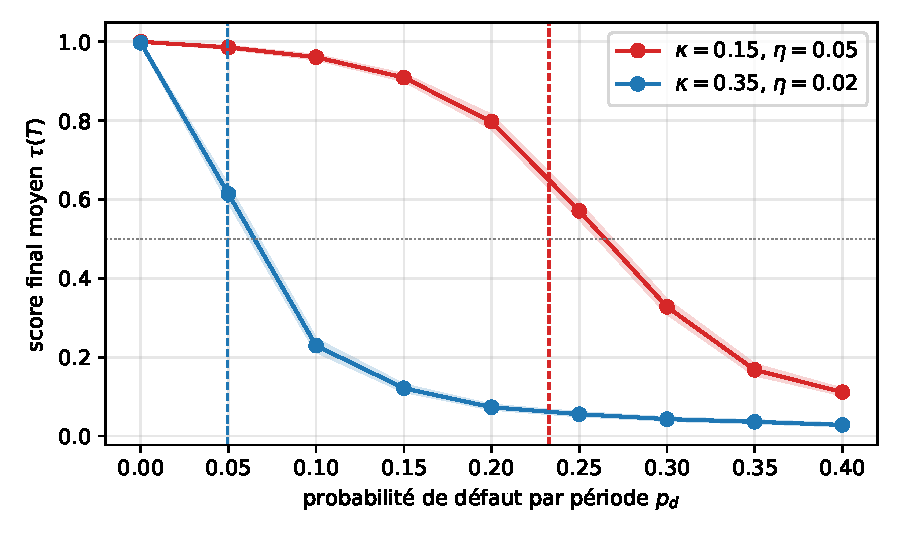
\includegraphics[width=0.7\textwidth]{figures/fig_E1_defaut.pdf}
\caption{E1 --- Score final des membres défaillants (IC 95\,\%, 200 graines).
Tirets~: seuil $p^\star_d$ (Prop.~\ref{prop:defaut})~; pointillés~: score initial.}
\label{fig:E1}
\end{figure}

Avec les paramètres de v1.1 ($p^\star_d=0{,}23$), des membres qui font défaut
une période sur sept terminent à $0{,}91$ $[0{,}90\,;\,0{,}92]$, et le score final
ne repasse sous le score initial qu'entre $p_d=0{,}25$ et $p_d=0{,}30$. Avec les
paramètres v2.1 ($p^\star_d=0{,}049$), un défaut une période sur vingt laisse
le score à $0{,}61$ $[0{,}60\,;\,0{,}63]$, légèrement au-dessus du score
initial comme le prédit la proximité du seuil, et un défaut une période sur
dix le ramène à $0{,}23$ $[0{,}22\,;\,0{,}25]$. Les deux seuils observés
concordent avec (\ref{eq:pstar}) au décalage près dû à la variation de $\bar q$
et aux bornes.

\subsection{E2 --- Collusion et probabilité d'audit}

Des coalitions de 8 et 12 membres sur 20 (40\,\% et 60\,\%) (Figure~\ref{fig:E2}).

\begin{figure}[h]
\centering
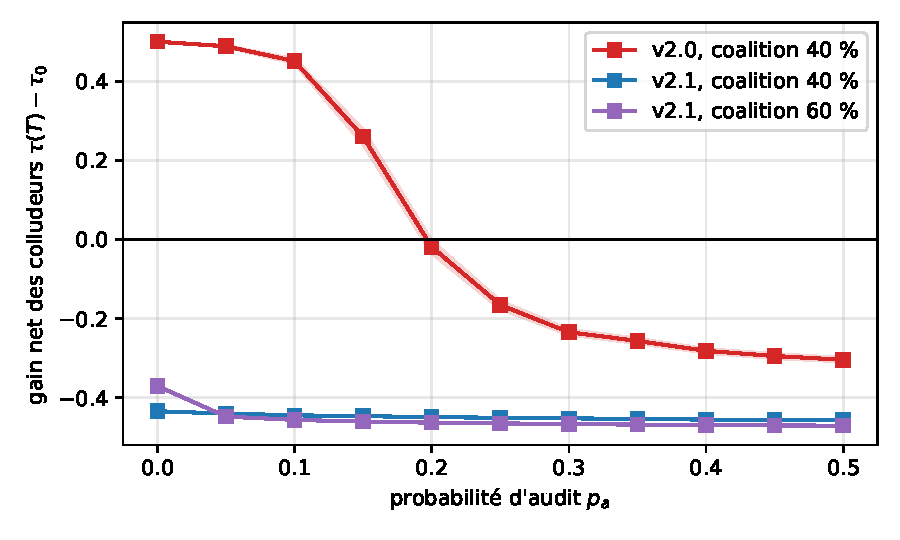
\includegraphics[width=0.7\textwidth]{figures/fig_E2_collusion.pdf}
\caption{E2 --- Gain net moyen d'une coalition en fonction de $p_a$ (IC 95\,\%, 200 graines).}
\label{fig:E2}
\end{figure}

Avec les paramètres de v1.1 (coalition de 40\,\%), le gain net vaut $+0{,}50$
sans audit, $+0{,}26$ $[0{,}24\,;\,0{,}28]$ à $p_a=0{,}15$, n'est plus
significativement non nul à $p_a=0{,}20$ ($-0{,}02$ $[-0{,}04\,;\,0{,}00]$) et
devient négatif au-delà, conformément au seuil de la
Proposition~\ref{prop:collusion} dans sa forme à sanction divisée
($0{,}146$ à $0{,}194$). Avec v2.1, la collusion est perdante \emph{pour toute
valeur de $p_a$, y compris nulle}~: $-0{,}43$ sans audit pour une coalition de
40\,\%, et $-0{,}37$ pour une coalition de 60\,\%. C'est la prédiction du
Corollaire~\ref{cor:sansaudit}~: avec $\delta/\eta=1$, la collusion exige
$\pi>1/2$, alors que la probabilité de capture vaut environ $0{,}04$ à 40\,\%
(E3) et $\pi(19,11,5,4)\approx0{,}27$ à 60\,\%. Dans v2.1, c'est la règle
d'inactivité, et non l'audit, qui dissuade la collusion minoritaire~;
l'audit reste la protection contre une coalition majoritaire et contre les
témoins négligents (E6).

\subsection{E3 --- Capture des panels}

Taux d'acceptation des signaux non conformes d'une coalition, $n=20$, sans
audit (Figure~\ref{fig:E3}).

\begin{figure}[h]
\centering
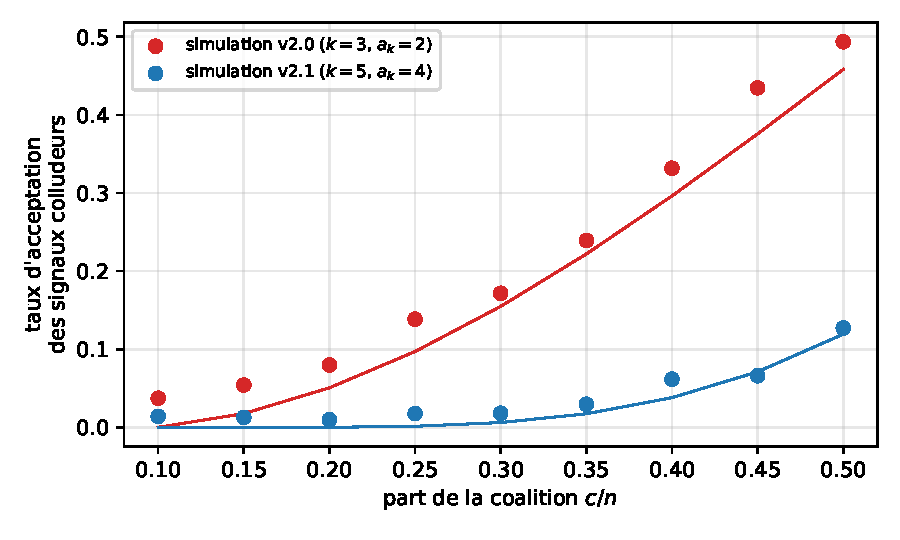
\includegraphics[width=0.7\textwidth]{figures/fig_E3_capture.pdf}
\caption{E3 --- Points~: simulation (100 graines)~; traits~: borne
hypergéométrique de la Proposition~\ref{prop:capture}.}
\label{fig:E3}
\end{figure}

Avec les paramètres de v1.1 ($k=3$, $a_k=2$), une coalition de 30\,\% voit
$17\,\%$ de ses signaux non conformes acceptés, et une coalition de moitié
$49\,\%$. Avec v2.1 ($k=5$, $a_k=4$), ces taux tombent à $1{,}8\,\%$ et
$12{,}7\,\%$. Les taux mesurés dépassent la borne (\ref{eq:hyper}) de l'effet
des erreurs des témoins honnêtes, à un écart d'échantillonnage près (45\,\%).

\subsection{E4 --- Comparaison des trois jeux de règles}

Vingt membres~: 10 honnêtes ($p_d=0{,}02$), 4 passagers clandestins,
6 colludeurs (Tableau~\ref{tab:E4}, Figure~\ref{fig:E4}).

\begin{table}[h]
\centering
\caption{E4 --- Score final moyen par groupe et taux d'erreur (200 graines~; IC 95\,\% entre crochets).}
\label{tab:E4}
\small
\begin{tabular}{lccc}
\toprule
& v1.1 & v2.0 & v2.1 \\
\midrule
Honnêtes & $0{,}99$ $[0{,}99\,;\,0{,}99]$ & $0{,}99$ $[0{,}99\,;\,0{,}99]$ & $0{,}91$ $[0{,}91\,;\,0{,}92]$ \\
Passagers clandestins & $0{,}07$ $[0{,}07\,;\,0{,}07]$ & $0{,}07$ $[0{,}07\,;\,0{,}07]$ & $0{,}06$ $[0{,}06\,;\,0{,}06]$ \\
Colludeurs & $0{,}58$ $[0{,}57\,;\,0{,}58]$ & $0{,}78$ $[0{,}77\,;\,0{,}80]$ & $0{,}06$ $[0{,}06\,;\,0{,}06]$ \\
\midrule
Fraude acceptée & $2{,}5\,\%$ & $19{,}1\,\%$ & $0{,}5\,\%$ \\
Rejet à tort & $8{,}6\,\%$ & $1{,}6\,\%$ & $3{,}7\,\%$ \\
Votes par signal & $3{,}0$ & $3{,}0$ & $5{,}3$ \\
Audits par signal & $0{,}00$ & $0{,}10$ & $0{,}09$ \\
\bottomrule
\end{tabular}
\end{table}

\begin{figure}[h]
\centering
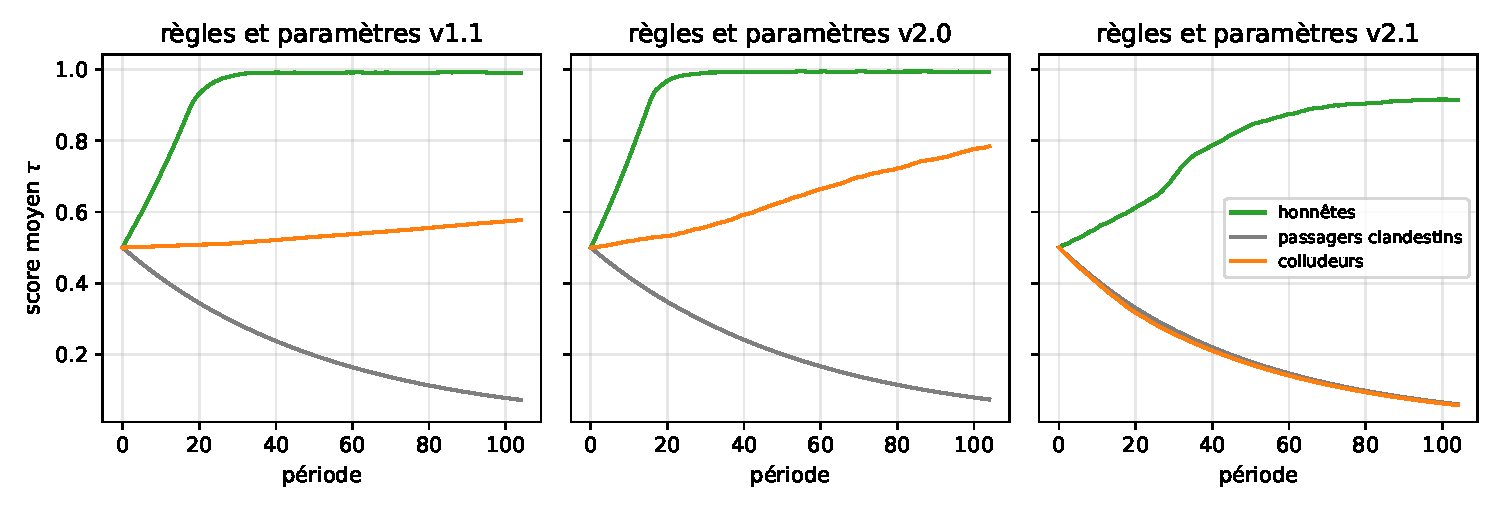
\includegraphics[width=\textwidth]{figures/fig_E4_comparaison.pdf}
\caption{E4 --- Trajectoires moyennes des scores par groupe.}
\label{fig:E4}
\end{figure}

Avec v1.1, les colludeurs terminent au-dessus de leur score initial
($0{,}58$)~: leurs rares contributions capturées ont un $q(s)$ supérieur à
$q_{\min}$ et ne sont jamais auditées, et l'unanimité rejette à tort $8{,}6\,\%$
des contributions honnêtes. Le modèle corrigé avec les paramètres de v1.1
(v2.0) est \emph{pire}~: $19\,\%$ des fraudes sont acceptées et les colludeurs
atteignent $0{,}78$, car l'approbation à 2 sur 3 multiplie la probabilité de
capture par quinze ($\pi\approx0{,}010\to0{,}155$), $p_a$ reste sous le seuil
et un signal rejeté ne coûte rien. Avec v2.1, les colludeurs tombent au niveau
des passagers clandestins ($0{,}06$) et $0{,}5\,\%$ des fraudes passent. La
contrepartie est un score moyen des honnêtes de $0{,}91$ au lieu de $0{,}99$~:
une pénalité de défaut plus sévère et $3{,}7\,\%$ de rejets à tort font payer
les défauts accidentels ($p_d=0{,}02$). Ce coût découle directement du choix de
$p^\star_d$ et peut être ajusté par le Corollaire~\ref{cor:kappa}.

\subsection{E5 --- Les témoins apportent-ils quelque chose~?}

Pour isoler l'apport des témoins, on compare v2.1 à deux références au même
$p_a=0{,}15$~: \emph{audit seul} (toute contribution est acceptée, avec
$q=1$, et seul l'audit sanctionne) et \emph{témoins sans responsabilité}
($\phi=\kappa_s=\eta_W=h=0$). Population~: 13 honnêtes, 3 fraudeurs isolés,
4 colludeurs (Tableau~\ref{tab:E5}).

\begin{table}[h]
\centering
\caption{E5 --- Comparaison aux références (200 graines).}
\label{tab:E5}
\small
\begin{tabular}{lccc}
\toprule
& audit seul & témoins sans resp. & v2.1 \\
\midrule
Honnêtes & $1{,}00$ $[1{,}00\,;\,1{,}00]$ & $1{,}00$ $[1{,}00\,;\,1{,}00]$ & $1{,}00$ $[1{,}00\,;\,1{,}00]$ \\
Fraudeurs isolés & $0{,}52$ $[0{,}50\,;\,0{,}54]$ & $0{,}06$ $[0{,}06\,;\,0{,}06]$ & $0{,}06$ $[0{,}06\,;\,0{,}06]$ \\
Colludeurs & $0{,}53$ $[0{,}51\,;\,0{,}55]$ & $0{,}06$ $[0{,}06\,;\,0{,}06]$ & $0{,}06$ $[0{,}06\,;\,0{,}06]$ \\
\midrule
Fraude acceptée & $84{,}9\,\%$ & $0{,}2\,\%$ & $0{,}2\,\%$ \\
Rejet à tort & $0{,}0\,\%$ & $3{,}8\,\%$ & $3{,}7\,\%$ \\
Votes par signal & $0{,}0$ & $5{,}0$ & $5{,}2$ \\
Audits par signal & $0{,}15$ & $0{,}09$ & $0{,}09$ \\
\bottomrule
\end{tabular}
\end{table}

\begin{figure}[h]
\centering
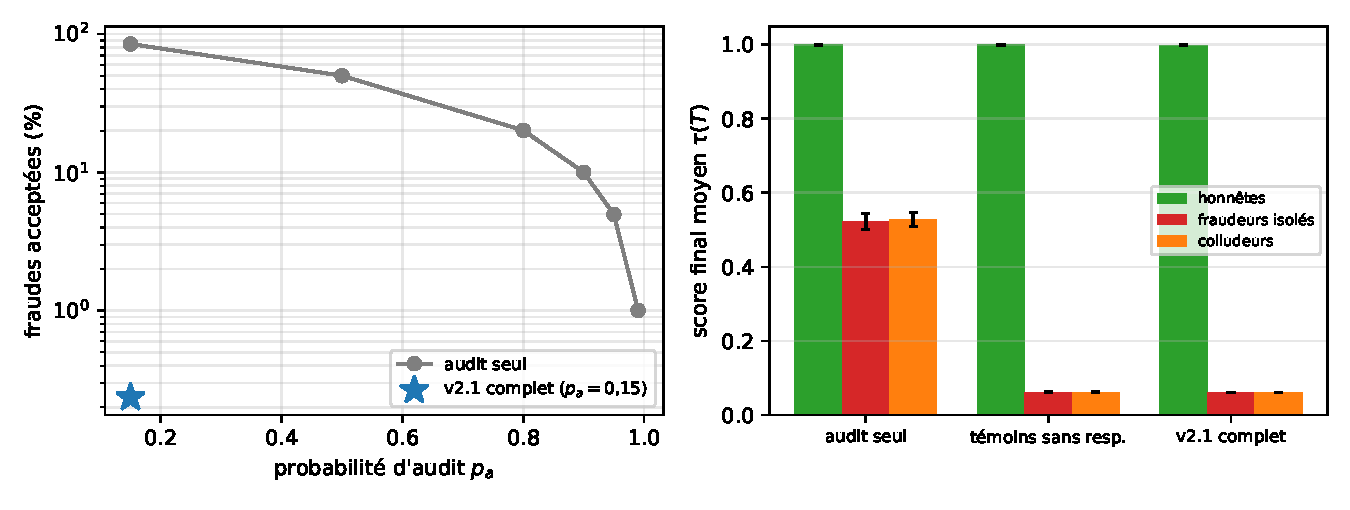
\includegraphics[width=0.95\textwidth]{figures/fig_E5_references.pdf}
\caption{E5 --- Gauche~: taux de fraudes acceptées par l'audit seul en fonction
de $p_a$ (échelle logarithmique), comparé à v2.1 à $p_a=0{,}15$. Droite~: score
final par groupe (IC 95\,\%).}
\label{fig:E5}
\end{figure}

L'audit seul, à $p_a=0{,}15$ (Figure~\ref{fig:E5}), laisse passer $85\,\%$ des fraudes~: les
fraudeurs conservent leur score initial. Pour ramener ce taux à $5\,\%$, il
faudrait auditer $95\,\%$ des contributions, et $99\,\%$ pour atteindre
$1\,\%$. Le panel de témoins obtient $0{,}24\,\%$ avec $5$ votes et $0{,}09$
audit par signal~: son intérêt dépend du coût relatif d'un vote et d'un audit,
et il est d'autant plus grand que l'audit est coûteux. En revanche, avec des
comportements fixés, les témoins \emph{sans} responsabilité font exactement
aussi bien que v2.1. Ce n'est pas surprenant~: la responsabilité agit sur les
incitations, que des agents à comportement fixé n'ont pas. E6 teste ce point.

\subsection{E6 --- Agents adaptatifs}

Les comportements fixés de E1--E5 ne testent pas les incitations. En E6, les
20 membres sont adaptatifs~: à chaque période, chacun choisit comme auteur entre
contribuer honnêtement (coût $c_h=0{,}01$) ou frauder, et comme témoin entre
vérifier (coût $c_v=0{,}001$) ou tamponner. Les choix sont appris par
$\varepsilon$-glouton ($\varepsilon=0{,}1$, pas $0{,}1$) sur le gain réalisé
de chaque rôle, sur 300 périodes et 50 graines. Outre les trois jeux de règles,
deux ablations de v2.1 sont testées~: sans signaux pièges ($h=0$), et sans
responsabilité ($\phi=\kappa_s=\eta_W=h=0$) (Figure~\ref{fig:E6}).

\begin{figure}[h]
\centering
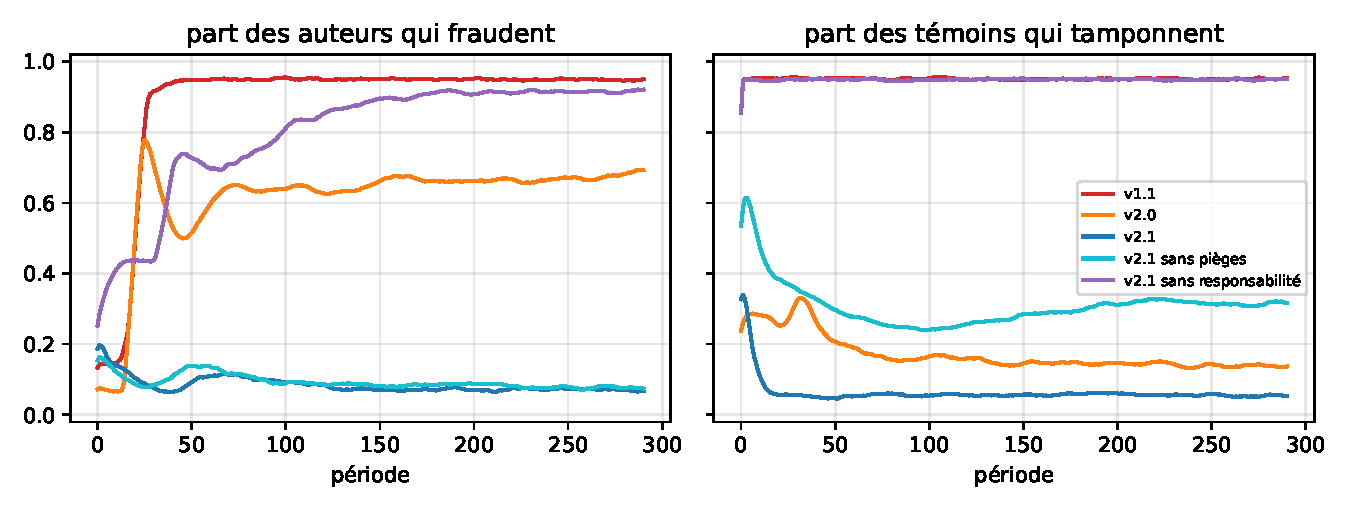
\includegraphics[width=0.95\textwidth]{figures/fig_E6_adaptatifs.pdf}
\caption{E6 --- Part des auteurs qui fraudent et des témoins qui tamponnent
(moyenne sur 50 graines, moyenne mobile sur 10 périodes). Le plancher
d'environ $0{,}05$ correspond à l'exploration $\varepsilon/2$.}
\label{fig:E6}
\end{figure}

Avec les règles de v1.1, le système s'effondre~: $95\,\%$ des auteurs fraudent
et $95\,\%$ des témoins tamponnent, et $87\,\%$ des fraudes sont acceptées.
Avec v2.0, les témoins vérifient majoritairement ($14\,\%$ de tampons), mais
$68\,\%$ des auteurs soumettent des signaux non conformes~: saturés à
$\tau=1$, ils ne gagnent rien à contribuer honnêtement, et un signal rejeté ne
les rend pas inactifs (Prop.~\ref{prop:plafond}). Avec v2.1, fraude et tampons
restent au niveau de l'exploration ($7{,}1\,\%$ $[6{,}3\,;\,8{,}2]$ et
$5{,}5\,\%$ $[5{,}0\,;\,6{,}0]$) et $2{,}1\,\%$ des fraudes passent. Les deux
ablations confirment le rôle de chaque composant~: sans signaux pièges,
$31\,\%$ des témoins tamponnent et $7{,}5\,\%$ des fraudes passent
(Prop.~\ref{prop:verif})~; sans responsabilité des témoins ni sanction de
l'auteur, le système s'effondre comme en v1.1 ($92\,\%$ de fraude, $95\,\%$ de
tampons, $83\,\%$ de fraudes acceptées). La responsabilité, inutile en
apparence avec des comportements fixés (E5), est ce qui empêche l'effondrement
lorsque les agents s'adaptent.

\subsection{E7 --- Sensibilité}

On fait varier un facteur à la fois autour de la configuration v2.1
(20 membres dont 30\,\% de colludeurs et 10\,\% de passagers clandestins,
100 graines). Le Tableau~\ref{tab:E7} donne le score final des honnêtes, le gain
net des colludeurs et les taux d'erreur.

\begin{table}[h]
\centering
\caption{E7 --- Sensibilité de v2.1 (100 graines par ligne).}
\label{tab:E7}
\small
\begin{tabular}{lcccc}
\toprule
Variante & honnêtes & gain colludeurs & fraude acceptée & rejet à tort \\
\midrule
Référence v2.1 & $0{,}92$ $[0{,}91\,;\,0{,}93]$ & $-0{,}44$ & $0{,}4\,\%$ & $3{,}7\,\%$ \\
$\sigma_{\text{obs}}=0{,}05$ & $0{,}93$ $[0{,}92\,;\,0{,}94]$ & $-0{,}44$ & $0{,}3\,\%$ & $1{,}2\,\%$ \\
$\sigma_{\text{obs}}=0{,}20$ & $0{,}70$ $[0{,}68\,;\,0{,}72]$ & $-0{,}45$ & $1{,}3\,\%$ & $14{,}1\,\%$ \\
$\sigma_{\text{obs}}=0{,}20$, $\theta=0{,}5$ & $0{,}73$ $[0{,}71\,;\,0{,}75]$ & $-0{,}46$ & $5{,}2\,\%$ & $3{,}9\,\%$ \\
$\varepsilon_a=0{,}05$ & $0{,}91$ $[0{,}90\,;\,0{,}92]$ & $-0{,}44$ & $0{,}4\,\%$ & $3{,}8\,\%$ \\
$\varepsilon_a=0{,}05$, sans contre-audit & $0{,}62$ $[0{,}59\,;\,0{,}65]$ & $-0{,}45$ & $0{,}4\,\%$ & $3{,}8\,\%$ \\
$\varepsilon_a=0{,}10$ & $0{,}87$ $[0{,}86\,;\,0{,}89]$ & $-0{,}44$ & $0{,}5\,\%$ & $3{,}8\,\%$ \\
$\varepsilon_a=0{,}10$, sans contre-audit & $0{,}36$ $[0{,}33\,;\,0{,}39]$ & $-0{,}48$ & $1{,}1\,\%$ & $3{,}2\,\%$ \\
$\tau_0=0{,}3$ & $0{,}92$ $[0{,}91\,;\,0{,}93]$ & $-0{,}26$ & $0{,}2\,\%$ & $3{,}8\,\%$ \\
$\tau_0=0{,}7$ & $0{,}92$ $[0{,}91\,;\,0{,}92]$ & $-0{,}62$ & $0{,}6\,\%$ & $3{,}8\,\%$ \\
$n=10$ & $0{,}92$ $[0{,}90\,;\,0{,}93]$ & $-0{,}44$ & $0{,}3\,\%$ & $3{,}6\,\%$ \\
$n=40$ & $0{,}91$ $[0{,}91\,;\,0{,}92]$ & $-0{,}44$ & $0{,}6\,\%$ & $2{,}4\,\%$ \\
$n=10$, panel non adaptatif & $0{,}36$ $[0{,}28\,;\,0{,}45]$ & $-0{,}44$ & $0{,}2\,\%$ & $2{,}1\,\%$ \\
coalition $10\,\%$ & $0{,}90$ $[0{,}89\,;\,0{,}91]$ & $-0{,}44$ & $0{,}6\,\%$ & $3{,}7\,\%$ \\
coalition $50\,\%$ & $0{,}93$ $[0{,}92\,;\,0{,}94]$ & $-0{,}46$ & $1{,}3\,\%$ & $3{,}7\,\%$ \\
$\theta=0{,}5$ & $0{,}92$ $[0{,}91\,;\,0{,}93]$ & $-0{,}45$ & $2{,}3\,\%$ & $1{,}1\,\%$ \\
$\theta=1$ & $0{,}88$ $[0{,}87\,;\,0{,}89]$ & $-0{,}44$ & $0{,}0\,\%$ & $12{,}0\,\%$ \\
$p_a=0{,}05$ & $0{,}92$ $[0{,}91\,;\,0{,}93]$ & $-0{,}44$ & $0{,}6\,\%$ & $3{,}8\,\%$ \\
$p_a=0{,}30$ & $0{,}92$ $[0{,}91\,;\,0{,}93]$ & $-0{,}44$ & $0{,}3\,\%$ & $3{,}7\,\%$ \\
$h=0$ & $0{,}92$ $[0{,}91\,;\,0{,}93]$ & $-0{,}44$ & $0{,}4\,\%$ & $3{,}8\,\%$ \\
$h=0{,}10$ & $0{,}91$ $[0{,}90\,;\,0{,}92]$ & $-0{,}44$ & $0{,}5\,\%$ & $3{,}8\,\%$ \\
\bottomrule
\end{tabular}
\end{table}

\begin{figure}[h]
\centering
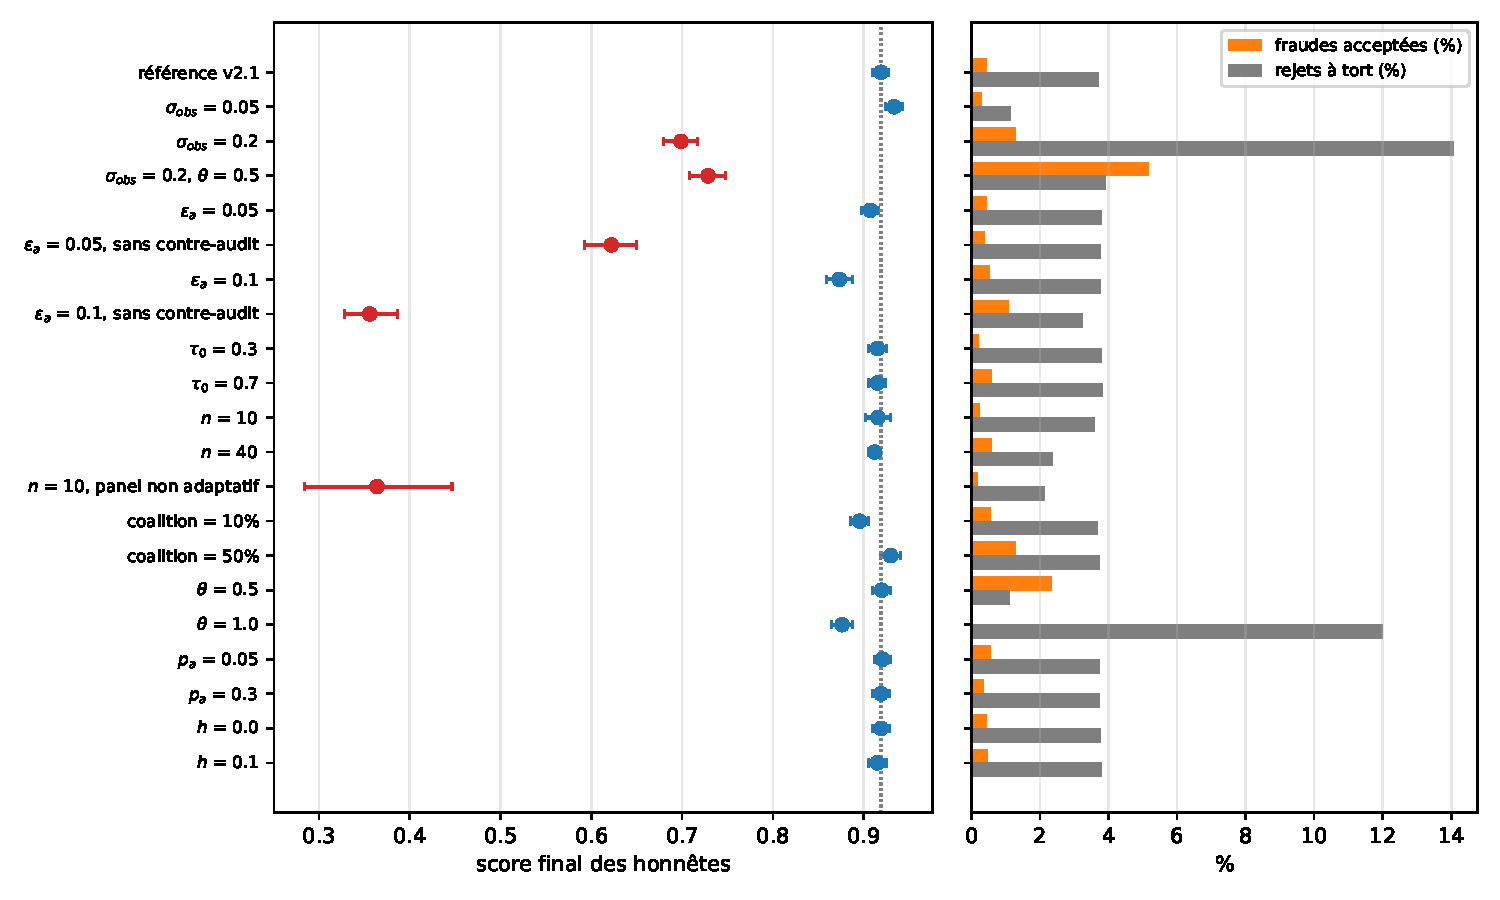
\includegraphics[width=\textwidth]{figures/fig_E7_sensibilite.pdf}
\caption{E7 --- Gauche~: score final des honnêtes par variante (IC 95\,\%~; en
rouge, sous $0{,}8$). Droite~: fraudes acceptées et rejets à tort.}
\label{fig:E7}
\end{figure}

Le mécanisme (Figure~\ref{fig:E7}) est stable vis-à-vis du score initial, de la taille du Node, de
la taille de la coalition jusqu'à 50\,\% ($1{,}3\,\%$ de fraudes acceptées), de
$p_a$ entre $0{,}05$ et $0{,}30$, et du taux de pièges. Deux défaillances,
révélées par une première version de cette analyse, ont conduit à modifier le
modèle~: sans contre-audit, une erreur d'audit de $5\,\%$ fait tomber les
honnêtes à $0{,}62$ et une erreur de $10\,\%$ à $0{,}36$, parce que chaque
sanction à tort retire $\phi\tau_w$ à tous les approbateurs et fait passer des
membres honnêtes sous $\tau_W$~; avec contre-audit, ils restent à $0{,}91$ et
$0{,}87$. Dans un Node de 10 membres, un panel de taille fixe fait tomber les
honnêtes à $0{,}36$ faute de témoins éligibles~; le panel adaptatif les
maintient à $0{,}92$.

La sensibilité restante concerne la précision des témoins. Avec
$\sigma_{\text{obs}}=0{,}20$, $14\,\%$ des contributions honnêtes sont
rejetées à tort et le score des honnêtes tombe à $0{,}70$. Abaisser $\theta$ à
$0{,}5$ ramène les rejets à tort à $3{,}9\,\%$ mais laisse passer $5{,}2\,\%$
des fraudes, et le score des honnêtes ne remonte qu'à $0{,}73$~: des témoins
imprécis approuvent eux-mêmes des signaux non conformes et sont sanctionnés.
Aucun réglage ne compense des témoins incapables de juger~; c'est une
condition d'applicabilité du mécanisme (Section~\ref{sec:discussion}).

% ════════════════════════════════════════════════════════════════
\section{Instanciation pour les tontines}
\label{sec:tontine}
% ════════════════════════════════════════════════════════════════

Dans une tontine, le signal principal --- une cotisation --- est un paiement,
vérifiable par un relevé de l'opérateur de paiement. L'audit y est donc
exhaustif et quasi gratuit ($p_a=1$, $\varepsilon_a\approx0$), et le panel de
témoins est superflu~: on pose $q=1$ pour toute cotisation versée à temps. Les
témoins restent utiles pour les engagements non vérifiables automatiquement
(par exemple une contribution en nature). Le risque propre aux tontines, le
départ d'un membre après réception du pot~\cite{anderson2009}, est traité par
deux règles.

\begin{regle}[Rotation par score]
Les rangs de réception du pot sont attribués par score décroissant~; à score
égal, par ancienneté.
\end{regle}

\begin{proposition}[Exposition]\label{prop:rotation}
Dans une tontine de $N$ membres et de cotisation $m$, le membre recevant le
pot au rang $r$ peut, en cessant de cotiser, s'approprier au plus $(N-r)\,m$.
Sous la règle de rotation par score, un membre de score strictement inférieur
à tous les autres reçoit le pot en dernier et son exposition est nulle.
\end{proposition}
\begin{proof}
Au rang $r$, le membre a versé $rm$ et reçu $Nm$~; il lui reste $(N-r)m$ à
verser. Au rang $N$, ce reste est nul.
\end{proof}

\begin{regle}[Parrainage et exclusion]
Un nouvel arrivant n'entre qu'avec un parrain de score au moins $\tau_W$. Il
démarre à $\tau_p$. Pendant une probation de $P$ périodes, chaque défaut du
filleul coûte $\psi$ au parrain. Un membre dont le score atteint 0 à la suite
d'un défaut est exclu~; sa réadmission exige un nouveau parrain.
\end{regle}

\begin{proposition}[Défauts avant exclusion]\label{prop:parrain}
Sous cette règle, une identité parrainée qui a obtenu au total $C$
contributions acceptées commet au plus $1+\lfloor(\tau_p+\eta\,C)/\kappa\rfloor$
défauts avant exclusion (hors récompenses de témoin), et chaque défaut pendant la probation coûte $\psi$ à
son parrain. Avec $\kappa=0{,}35$ et $\tau_p\le0{,}35$, une identité qui fait
défaut avant toute contribution est exclue au premier défaut.
\end{proposition}
\begin{proof}
Le score cumulé disponible est au plus $\tau_p+\eta C$~; chaque défaut en
retire $\kappa$ tant que le score reste positif, et le défaut qui le ramène à 0
entraîne l'exclusion.
\end{proof}

Le parrainage transfère le coût d'une identité nouvelle --- et donc des attaques
Sybil et du blanchiment par changement d'identité --- sur un membre établi,
qui est ainsi incité à filtrer les candidats. C'est la logique de la
responsabilité conjointe du microcrédit~\cite{besley1995,ghatak1999}, et
celle des garants dans les tontines traditionnelles. Combinée à la rotation
par score, elle place les nouveaux venus en fin de rotation, où leur exposition
est nulle, jusqu'à ce qu'ils aient construit un historique.

% ════════════════════════════════════════════════════════════════
\section{Discussion}
% ════════════════════════════════════════════════════════════════

\label{sec:discussion}
\paragraph{Ce que les résultats établissent.} Le mécanisme révisé admet des
conditions fermées que la simulation confirme, et ces conditions permettent de
le calibrer. Chaque composant a un rôle identifiable~: le panel filtre les
fraudes (E3, E5)~; la règle d'inactivité rend la collusion minoritaire
perdante même sans audit (Cor.~\ref{cor:sansaudit}, E2) et maintient
l'incitation au score maximal (Prop.~\ref{prop:plafond}, E6)~; la
responsabilité des témoins et les signaux pièges empêchent la validation sans
vérification (Prop.~\ref{prop:verif}, E6)~; l'audit, doublé d'un contre-audit,
protège contre les coalitions majoritaires sans pénaliser les honnêtes (E7).

\paragraph{Ce que coûtent les témoins.} Le panel remplace un audit
quasi exhaustif par cinq votes par signal. Il n'est pertinent que si un vote
coûte nettement moins qu'un audit.

\paragraph{Condition d'applicabilité.} Le mécanisme suppose des témoins
capables de juger la conformité avec une bonne précision (E7). Lorsque ce n'est
pas le cas, il vaut mieux ne noter que des contributions vérifiables
automatiquement --- ce qui est précisément le cas des tontines
(Section~\ref{sec:tontine}), où les témoins deviennent superflus.

\paragraph{Portée.} Les versions précédentes présentaient \CTP{} comme
universel. Les résultats montrent plutôt un cadre paramétrable dont les
paramètres pertinents ($\kappa/\eta$, $\delta/\eta$, $k$, $\theta$, $h$)
dépendent de la nature des contributions, de la précision des témoins et du
coût d'une identité~; chaque instanciation doit être calibrée, puis évaluée sur
des données réelles.

% ════════════════════════════════════════════════════════════════
\section{Limites}
\label{sec:limites}
% ════════════════════════════════════════════════════════════════

\begin{itemize}
  \item \textbf{Aucune donnée réelle.} Les distributions de qualité, de défaut
    et les coûts $c_h$, $c_v$ sont choisis. L'Annexe~\ref{app:collecte} décrit
    le protocole de collecte nécessaire.
  \item \textbf{Apprentissage simple.} Les agents de E6 apprennent
    indépendamment~; une coalition qui apprendrait conjointement, ou un
    adversaire qui chercherait à reconnaître les signaux pièges, n'est pas
    modélisé. L'indiscernabilité des pièges (Hyp.~\ref{h:tirage}) est
    une exigence de conception, non un acquis.
  \item \textbf{Précision des témoins.} Le mécanisme se dégrade lorsque les
    témoins jugent mal (E7)~; mesurer cette précision est un préalable à toute
    application à des contributions non vérifiables.
  \item \textbf{Organisation de l'audit.} Le modèle fixe $p_a$ et
    $\varepsilon_a$ sans préciser qui audite~; hors du cas des paiements, la
    question reste ouverte.
  \item \textbf{Utilité.} L'analyse stratégique suppose une utilité linéaire en
    score~; la forme réelle des droits attachés au score n'est pas modélisée.
  \item \textbf{Relecture.} Ce document n'a pas été relu par des pairs.
\end{itemize}

% ════════════════════════════════════════════════════════════════
\section{Conclusion}
% ════════════════════════════════════════════════════════════════

Nous avons reformulé le mécanisme de réputation à témoins responsables de
\CTP{} en un modèle cohérent, établi des conditions fermées pour sa tolérance au
défaut, sa résistance à la collusion, l'incitation à contribuer et à vérifier,
et son coût d'entrée, puis dérivé de ces conditions un jeu de paramètres.
Évalué contre des références, avec des agents adaptatifs et sous une analyse de
sensibilité, le mécanisme recalibré rend la fraude non rentable là où les règles
d'origine s'effondrent. Deux défaillances révélées en cours d'évaluation ont été
corrigées~; une condition d'applicabilité --- la précision des témoins --- demeure.
Pour les tontines, l'instanciation proposée n'utilise pas de témoins mais
repose sur des paiements vérifiables, une rotation par score et le parrainage.
La prochaine étape est empirique~: la collecte de données décrite en
Annexe~\ref{app:collecte}.

\paragraph{Reproductibilité.} Le script
\texttt{simulations-v2.0/ctp\_core\_v2\_experiments.py}
produit l'ensemble des figures, tableaux et le fichier
\texttt{resultats\_v2.json}, avec des graines fixées.

% ════════════════════════════════════════════════════════════════
\appendix
\section{Erratum des versions v0.1 et v1.1}
\label{app:erratum}
% ════════════════════════════════════════════════════════════════

\begin{enumerate}
  \item \textbf{Condition anti-collusion (Prop.~4.2).} La v1.1 affirme que
    $\phi\ge3\eta$ suffit pour $\tau_w\ge0{,}3$ et $\Prob(\text{détection})\ge0{,}15$.
    L'inégalité énoncée, $\phi>\eta q/(\tau_w\Prob)$, exige alors
    $\phi>22{,}2\,\eta q$~; avec $\phi=3\eta$ elle ne tient que pour $q<0{,}135$.
    De plus, le gain attribué au témoin colludeur n'existait pas dans le modèle.
  \item \textbf{Absence d'incitation à valider.} Corrigée par $R_i$.
  \item \textbf{Audit ciblé sur $q(s)<q_{\min}$.} Les coalitions bien notées
    n'étaient jamais auditées. Corrigé par un audit uniforme.
  \item \textbf{Aucune sanction de l'auteur.} Corrigé par $S_i$.
  \item \textbf{Sanction des témoins divisée par $|\mathcal{W}(s)|$.} Diluait la
    responsabilité. Corrigé.
  \item \textbf{Facteur de consensus constant.} $\min(|\mathcal{W}(s)|/k_j,1)=1$
    pour tout signal accepté. Remplacé par $|\mathcal{A}(s)|/k$ avec $a_k<k$.
  \item \textbf{Convergence (Prop.~3.2).} $\epsilon$ non défini~; remplacée par
    la Proposition~\ref{prop:sat}.
  \item \textbf{Inactivité.} Soumettre un signal suffisait à rester actif, ce qui
    supprime l'incitation au score maximal (Prop.~\ref{prop:plafond}, E6).
  \item \textbf{Indice de difficulté $\rho_j$.} Division par $\tau_{\min}$, nul
    dès qu'un membre atteint 0~; symbole $\rho$ utilisé pour deux objets.
    Reformulé en Annexe~\ref{app:extensions}.
  \item \textbf{Validation par simulation.} Avec $n=12$, $k=3$, unanimité et un
    seul complice, la probabilité de succès d'une collusion était nulle~;
    l'audit du code utilisait la qualité réelle, inconnue du protocole~; le
    score honnête de $1{,}000$ reflète la saturation.
  \item \textbf{Résistance Sybil.} Affirmée sans démonstration. Remplacée par
    les Propositions~\ref{prop:sybil} et~\ref{prop:parrain}.
  \item \textbf{Coûts gas.} Estimations non mesurées~; retirées.
  \item \textbf{Références.} Les citations de la v0.1 publiée apparaissaient
    comme \og{}[?]\fg{}.
\end{enumerate}

\section{Protocole de collecte de données}
\label{app:collecte}

La calibration empirique requiert, pour chaque tontine suivie et chaque
membre-période~: la cotisation due, la date et le montant versés, le rang de
réception du pot, les départs et exclusions, ainsi que les caractéristiques du
groupe (taille, montant, périodicité, ancienneté, existence de garants).

\paragraph{Taille d'échantillon.} Pour estimer un taux de défaut de l'ordre de
$5\,\%$ à $\pm2$ points près avec 95\,\% de confiance, il faut environ
$1{,}96^2\times0{,}05\times0{,}95/0{,}02^2\approx456$ observations
membre-période indépendantes. Les observations d'un même membre étant
corrélées, un effet de plan de 2 porte ce besoin à environ 900, soit par
exemple trois tontines de quinze membres suivies pendant vingt périodes.

\paragraph{Paramètres visés.} Le taux de défaut observé $p_d$ et la tolérance
effective des groupes (nombre de défauts avant exclusion) fixent $p^\star_d$,
donc $\kappa/\eta$ par le Corollaire~\ref{cor:kappa}~; la fréquence des départs
après réception du pot permet de tester la Proposition~\ref{prop:rotation}.

\paragraph{Éthique.} Consentement éclairé des membres, anonymisation des
identités et des montants avant analyse, restitution des résultats aux groupes.

\section{Extensions hors périmètre}
\label{app:extensions}

La v1.1 définissait un indice de difficulté
$\rho_j=k_j\bar\tau_j/(k_{\min}\tau_{\min})$, indéfini lorsque $\tau_{\min}=0$.
Une forme bien définie est
$\rho_j=(k_j/k_{\min})\cdot(\varepsilon+\bar\tau_j)/(\varepsilon+\bar\tau_{\mathcal M})$,
avec $\bar\tau_{\mathcal M}$ le score moyen de l'ensemble des Nodes et
$\varepsilon>0$. Cet indice, le score global et la portabilité inter-Nodes ne
sont pas analysés ici et ne doivent pas être considérés comme validés.

\section{Table des symboles}

\begin{center}
\small
\begin{tabular}{cl}
\toprule
$\tau_i(t)$ & score du membre $i$ \\
$k$, $a_k$, $\theta$ & taille du panel, approbations requises, fraction requise \\
$\mathcal{P}(s)$, $\mathcal{A}(s)$ & panel et approbateurs du signal $s$ \\
$q(s)$, $Q(s)$ & qualité mesurée, conformité réelle \\
$\eta,\eta_W$ & gain de l'auteur, récompense des témoins \\
$\kappa,\kappa_s$ & pénalités de défaut et de sanction de l'auteur \\
$\delta$, $\phi$ & dépréciation, responsabilité des témoins \\
$p_a$, $\varepsilon_a$, $h$ & probabilité et erreur d'audit, taux de pièges \\
$\tau_W,\tau_0,\tau_p$ & seuil d'éligibilité, score des fondateurs, des filleuls \\
$c_h$, $c_v$ & coûts d'une contribution honnête, d'une vérification \\
$p^\star_d, p^\star_a$ & seuils de tolérance au défaut et d'audit \\
$\pi$ & probabilité de capture d'un panel \\
$\psi$, $P$ & pénalité du parrain, durée de probation \\
\bottomrule
\end{tabular}
\end{center}

% ════════════════════════════════════════════════════════════════
\begin{thebibliography}{99}
\small

\bibitem{abebe2022}
R.~Abebe, A.~Eck, C.~Ikeokwu et S.~Taggart.
An algorithmic introduction to savings circles.
In \emph{Proc. AAAI Conference on Artificial Intelligence}, 2022.

\bibitem{anderson2009}
S.~Anderson, J.-M. Baland et K.~O. Moene.
Enforcement in informal saving groups.
\emph{Journal of Development Economics}, 90(1)~:14--23, 2009.

\bibitem{ardener1964}
S.~Ardener.
The comparative study of rotating credit associations.
\emph{Journal of the Royal Anthropological Institute}, 94(2)~:201--229, 1964.

\bibitem{besley1995}
T.~Besley et S.~Coate.
Group lending, repayment incentives and social collateral.
\emph{Journal of Development Economics}, 46(1)~:1--18, 1995.

\bibitem{besley1993}
T.~Besley, S.~Coate et G.~Loury.
The economics of rotating savings and credit associations.
\emph{American Economic Review}, 83(4)~:792--810, 1993.

\bibitem{buterin2021}
V.~Buterin.
Moving beyond coin voting governance.
\url{https://vitalik.ca/general/2021/08/16/voting3.html}, 2021.

\bibitem{cheng2005}
A.~Cheng et E.~Friedman.
Sybilproof reputation mechanisms.
In \emph{Proc. ACM SIGCOMM Workshop on Economics of Peer-to-Peer Systems
(P2PECON)}, p.~128--132, 2005.

\bibitem{dellarocas2003}
C.~Dellarocas.
The digitization of word of mouth: promise and challenges of online feedback
mechanisms.
\emph{Management Science}, 49(10)~:1407--1424, 2003.

\bibitem{douceur2002}
J.~R. Douceur.
The Sybil attack.
In \emph{Peer-to-Peer Systems (IPTPS)}, LNCS 2429, p.~251--260. Springer, 2002.

\bibitem{friedman2001}
E.~J. Friedman et P.~Resnick.
The social cost of cheap pseudonyms.
\emph{Journal of Economics \& Management Strategy}, 10(2)~:173--199, 2001.

\bibitem{fudenberg1986}
D.~Fudenberg et E.~Maskin.
The folk theorem in repeated games with discounting or with incomplete
information.
\emph{Econometrica}, 54(3)~:533--554, 1986.

\bibitem{ghatak1999}
M.~Ghatak et T.~W. Guinnane.
The economics of lending with joint liability: theory and practice.
\emph{Journal of Development Economics}, 60(1)~:195--228, 1999.

\bibitem{handa1999}
S.~Handa et C.~Kirton.
The economics of rotating savings and credit associations: evidence from the
Jamaican `Partner'.
\emph{Journal of Development Economics}, 60(1)~:173--194, 1999.

\bibitem{hoffman2009}
K.~Hoffman, D.~Zage et C.~Nita-Rotaru.
A survey of attack and defense techniques for reputation systems.
\emph{ACM Computing Surveys}, 42(1)~:1--31, 2009.

\bibitem{josang2007}
A.~Jøsang, R.~Ismail et C.~Boyd.
A survey of trust and reputation systems for online service provision.
\emph{Decision Support Systems}, 43(2)~:618--644, 2007.

\bibitem{kamvar2003}
S.~D. Kamvar, M.~T. Schlosser et H.~Garcia-Molina.
The EigenTrust algorithm for reputation management in P2P networks.
In \emph{Proc. 12th International World Wide Web Conference}, p.~640--651, 2003.

\bibitem{kandori1992}
M.~Kandori.
Social norms and community enforcement.
\emph{Review of Economic Studies}, 59(1)~:63--80, 1992.

\bibitem{kleros2019}
C.~Lesaege, F.~Ast et W.~George.
Kleros: short paper v1.0.7.
\url{https://kleros.io/assets/whitepaper.pdf}, 2019.

\bibitem{luu2015}
L.~Luu, J.~Teutsch, R.~Kulkarni et P.~Saxena.
Demystifying incentives in the consensus computer.
In \emph{Proc. ACM SIGSAC Conference on Computer and Communications Security
(CCS)}, p.~706--719, 2015.

\bibitem{marsh1994}
S.~P. Marsh.
\emph{Formalising Trust as a Computational Concept}.
Thèse de doctorat, University of Stirling, 1994.

\bibitem{ostrom1990}
E.~Ostrom.
\emph{Governing the Commons: The Evolution of Institutions for Collective
Action}. Cambridge University Press, 1990.

\bibitem{resnick2000}
P.~Resnick, K.~Kuwabara, R.~Zeckhauser et E.~Friedman.
Reputation systems.
\emph{Communications of the ACM}, 43(12)~:45--48, 2000.

\bibitem{teutsch2017}
J.~Teutsch et C.~Reitwießner.
A scalable verification solution for blockchains.
arXiv:1908.04756, 2017.

\bibitem{weyl2022}
E.~G. Weyl, P.~Ohlhaver et V.~Buterin.
Decentralized society: finding Web3's soul.
SSRN 4105763, 2022.

\bibitem{xiong2004}
L.~Xiong et L.~Liu.
PeerTrust: supporting reputation-based trust for peer-to-peer electronic
communities.
\emph{IEEE Transactions on Knowledge and Data Engineering}, 16(7)~:843--857, 2004.

\end{thebibliography}
\end{document}
